\newpage
\def\thoigian{90}%--Thời gian
\de{Đề số 3}{Chương I. Hàm số lượng giác và phương trình lượng giác}




\begin{center}
	\textbf{PHẦN 1 - CÂU TRẮC NGHIỆM BỐN PHƯƠNG ÁN}
\end{center}
\Opensolutionfile{ans}[ans/ans-TN-1D1-DE3]
% Góc Lượng giác 2
\begin{ex}[Trích đề thi HKI - THPT Chuyên Hùng Vương - năm học 2022-2023]%[1D1N1-1]%[Dự án D - đợt 4 NH25-26- Nguyễn Trần Anh Tuấn]
	Gọi $M$ là điểm trên nửa đường tròn đơn vị sao cho $\widehat{xOM}=0^\circ$. Tọa độ của điểm $M$ là
	\choice
	{\True $(1; 0)$}
	{$(0; 1)$}
	{$(0;-1)$}
	{$(-1; 0)$}
	\loigiai{
		Ta có $\cos 0^\circ =1$, $\sin 0^\circ=0$ nên tọa độ điểm $M$ là $(1;0)$.
	}
\end{ex}
\begin{ex}[Trích đề thi HKI - THPT Chuyên Hùng Vương - năm học 2022-2023]%[1D1H1-2]%[Dự án D - đợt 4 NH25-26- Nguyễn Trần Anh Tuấn]
	Đổi số đo góc $\alpha=105^{\circ}$ sang radian ta được
	\choice
	{$\alpha=\dfrac{\pi}{8}$}
	{\True $\alpha=\dfrac{7 \pi}{12}$}
	{$\alpha=\dfrac{5 \pi}{8}$}
	{$\alpha=\dfrac{9 \pi}{12}$}
	\loigiai{
		Ta có $\alpha =\dfrac{105 \pi}{180}=\dfrac{7\pi}{12}$.
	}
\end{ex}
% Giá trị LG 2
\begin{ex}[Trích đề thi HKI -  Chuyên Võ Nguyên Giáp, Quảng Bình - năm học 2022-2023]%[1D1N2-2]%[Dự án D - đợt 4 NH25-26- Nguyễn Trần Anh Tuấn]
	Cho góc $\alpha$ thỏa mãn $90^\circ <\alpha <180^\circ$. Khẳng định nào sau đây đúng?
	\choice
	{$\cos\alpha>0$}
	{\True $\sin\alpha>0$}
	{$\tan\alpha>0$}
	{$\cot\alpha>0$}
	\loigiai
	{Vì $90^\circ <\alpha <180^\circ$ nên $\sin\alpha>0$, $\cos\alpha<0$, $\tan\alpha<0$ và $\cot\alpha<0$.}
\end{ex}
\begin{ex}[Trích đề thi HKI -  Sở giáo dục Bắc Giang - năm học 2022-2023]%[1D1N2-2]%[Dự án D - đợt 4 NH25-26- Nguyễn Trần Anh Tuấn]
	Tính giá trị của biểu thức $P=\sin 75^{\circ}+\sin 55^{\circ}-\cos 15^{\circ}+\cos 145^{\circ}+\cos 180^{\circ}$.
	\choice
	{$P=0$}
	{\True $P=-1$}
	{$P=1$}
	{$P=2$}
	\loigiai{
		Ta có $P=\sin 75^{\circ}+\sin 55^{\circ}-\sin 75^{\circ}-\sin 55^{\circ}+\cos 180^{\circ}=\cos180^\circ=-1$.
	}
\end{ex}
% Công thức LG 3
\begin{ex}[Trích đề thi HKI - THPT Trần Phú, TpHCM - năm học 2023-2024]%[1D1H3-2]%[Dự án D - đợt 4 NH25-26- Nguyễn Trần Anh Tuấn]
	Cho $\sin a=\dfrac{5}{13}$, $\cos a=\dfrac{12}{13}$; $\sin b=\dfrac{4}{5}$ và $\cos b =\dfrac{3}{5}$. Khẳng định nào sau đây đúng?
	\choice
	{$\cos (a+b)=\dfrac{56}{65}$}
	{\True  $\cos (a+b)=\dfrac{16}{65}$}
	{$\cos (a+b)=-\dfrac{33}{65}$}
	{$\cos (a+b)=\dfrac{63}{65}$}
	\loigiai{
		Ta có $\cos (a+b) =\cos a \cos b - \sin a\sin b = \dfrac{12}{13} \cdot \dfrac{3}{5} -\dfrac{5}{13} \cdot  \dfrac{4}{5}=\dfrac{16}{65}$.
	}
\end{ex}
\begin{ex}[Trích đề thi HKI - THPT Trần Phú, TpHCM - năm học 2023-2024]%[1D1H3-5]%[Dự án D - đợt 4 NH25-26- Nguyễn Trần Anh Tuấn]
	Khẳng định nào sau đây \textbf{sai}?
	\choice
	{\True $\sin5a\sin3a=\dfrac{1}{2}(\cos8a-\cos2a)$, $\forall a\in\mathbb{R}$}
	{$\sin5a+\sin3a=2\sin4a\cos a$, $\forall a\in\mathbb{R}$}
	{$\cos4a=2\cos^2 2a-1$, $\forall a\in\mathbb{R}$}
	{$\sin a=2\sin\dfrac{a}{2}\cos\dfrac{a}{2}$, $\forall a\in\mathbb{R}$}
	\loigiai{
		Ta có $\sin5a \sin3a = \dfrac{1}{2} \left[ \cos(5a - 3a) - \cos(5a + 3a) \right] = \dfrac{1}{2} \left[ \cos2a - \cos8a \right]$.
	}
\end{ex}
\begin{ex}[Trích đề thi HKI - Chuyên Hùng Vương - Phú Thọ - năm học 2022-2023]%[1D1H3-2]%[Dự án D - đợt 4 NH25-26- Nguyễn Trần Anh Tuấn]
	Nếu hai góc $a$ và $b$ có $\tan a=\dfrac{1}{3}$ và $\tan b=\dfrac{1}{2}$ thì giá trị của $\tan (a-b)$ bằng
	\choice
	{$\dfrac{1}{7}$}
	{\True $\dfrac{-1}{7}$}
	{$1$}
	{$\dfrac{-1}{5}$}
	\loigiai{
		Áp dụng công thức cộng ta có $\tan{\left(a-b\right)}=\dfrac{\tan{a}-\tan{b}}{1+\tan{a}\cdot\tan{b}}=\dfrac{\dfrac{1}{3}-\dfrac{1}{2}}{1+\dfrac{1}{3}\cdot\dfrac{1}{2}}=-\dfrac{1}{7}$.
	}
\end{ex}
% Hàm số LG 3
\begin{ex}%[1D1H4-2]%[Dự án D - đợt 4 NH25-26- Nguyễn Trần Anh Tuấn]
	Hàm số nào sau đây có tập xác định là $\mathbb{R}$?
	\choice
	{$y=\tan 2 x+1$}
	{$y=2 \cos \sqrt{x}$}
	{$y=\dfrac{\cot x}{\sin ^2 x+1}$}
	{\True $y=\sqrt{1-\cos 2 x}$}
	\loigiai{
		Ta có $\cos 2x\le 1 \Leftrightarrow 1-\cos 2x\geq 0$, với mọi $x$.\\ 
		Vậy hàm số $y=\sqrt{1-\cos 2 x}$ có tập xác định là $\mathscr{D}=\mathbb{R}$.}
\end{ex}
\begin{ex}%[1D1H4-4]%[Dự án D - đợt 4 NH25-26- Nguyễn Trần Anh Tuấn]
	Trong các hàm số sau, hàm số nào là hàm số chẵn?
	\choice
	{$f(x)=\sin x+\cos x$}
	{\True $f(x)=\sin |x|+\cos x$}
	{$f(x)=\tan 2 x$}
	{$f(x)=\cot x$}
	\loigiai{
		\allowdisplaybreaks
		\begin{itemize}
			\item Xét hàm số $f(x)=\sin x+\cos x$.\\
			Tập xác định $ \mathscr{D}=\mathbb{R} $.\\
			$ \forall x \in \mathscr{D} \Rightarrow \heva{&-x \in \mathscr{D}\\&f(-x)=\sin (-x)+\cos (-x)=-\sin x +\cos x \Rightarrow f(-x) \neq f(x),\,f(-x) \neq -f(x).}$\\
			Suy ra hàm số $f(x)=\sin x+\cos x$ không chẵn, không lẻ.
			\item Xét hàm số $f(x)=\cot x$.\\
			Tập xác định $ \mathscr{D}=\mathbb{R} \setminus \left\{ k\pi \right\}$.\\
			$ \forall x \in \mathscr{D} \Rightarrow \heva{&-x \in \mathscr{D}\\&f(-x)=\cot (-x)=-\cot  x=-f(x).}$\\
			Suy ra hàm số $f(x)=\cot x$ là hàm số lẻ.
			\item Xét hàm số $f(x)=\tan 2 x$.\\
			Tập xác định $ \mathscr{D}=\mathbb{R} \setminus \left\{ \dfrac{\pi}{4}+k \dfrac{\pi}{2} \right\}$.\\
			$ \forall x \in \mathscr{D} \Rightarrow \heva{&-x \in \mathscr{D}\\&f(-x)=\tan (-2x)=-\tan 2x=-f(x).}$\\
			Suy ra hàm số $f(x)=\tan 2 x$ là hàm số lẻ.
			\item Xét hàm số $f(x)=\sin |x|+\cos x$.\\
			Tập xác định $ \mathscr{D}=\mathbb{R} $.\\
			$ \forall x \in \mathscr{D} \Rightarrow \heva{&-x \in \mathscr{D}\\&f(-x)=\sin |-x|+\cos (-x)=\sin |x|+\cos x=f(x).}$\\
			Suy ra hàm số $f(x)=\sin |x|+\cos x$ là hàm số chẵn.
		\end{itemize}
	}
\end{ex}
\begin{ex}[Trích đề thi HKI -  Chuyên Võ Nguyên Giáp, Quảng Bình - năm học 2022-2023]%[1D1N4-7]%[Dự án D - đợt 4 NH25-26- Nguyễn Trần Anh Tuấn]
	Cho đồ thị hàm số $y=\sin x$ trên đoạn $\left[-\pi;2\pi \right]$, giá trị của $x$ để hàm số $y=\sin x$ nhận giá trị bằng $1$ là
	\begin{center}
		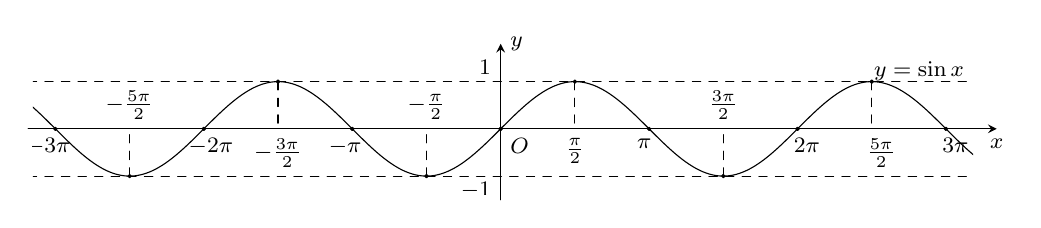
\begin{tikzpicture}[scale=0.6,>=stealth, font=\footnotesize, line join=round, line cap=round]
			\def\xmin{-10} \def\xmax{10.5} \def\ymin{-1.5} \def\ymax{1.8}
			\draw[->] (\xmin,0)--(\xmax,0) node [below]{$x$};
			\draw[->] (0,\ymin)--(0,\ymax) node [right]{$y$};
			\node at (0,0) [below right]{$O$};
			\clip (\xmin+0.1,\ymin+0.1) rectangle (\xmax-0.5,\ymax-0.1);
			\draw[smooth,samples=400,domain=\xmin:\xmax] plot(\x,{sin(\x r)});
			\draw[dashed] (\xmin,1)--(\xmax,1) (\xmin,-1)--(\xmax,-1);
			\foreach \x in {-3*pi,-2.5*pi,-2*pi,-1.5*pi,-pi,-0.5*pi,0}
			{\draw[fill=black] (\x,sin \x*180/pi) circle (1pt);
				\draw[dashed] (\x,sin \x*180/pi)--(\x,0);
				\draw[fill=black] (-\x,sin -\x*180/pi) circle (1pt);
				\draw[dashed] (-\x,sin -\x*180/pi)--(-\x,0);}
			\node at (0,1.3) [left]{$1$};
			\node at (0,-1.3) [left]{$-1$};
			\node at (-2*pi+0.15,0) [below]{$-2\pi$};
			\node at (-3*pi-0.15,0) [below]{$-3\pi$};
			\node at (-2.5*pi,0) [above]{$-\frac{5\pi}{2}$};
			\node at (-1.5*pi,0) [below]{$-\frac{3\pi}{2}$};
			\node at (-pi-0.15,0) [below]{$-\pi$};
			\node at (-0.5*pi,0) [above]{$-\frac{\pi}{2}$};
			\node at (0.5*pi,0) [below]{$\frac{\pi}{2}$};
			\node at (pi-0.1,0) [below]{$\pi$};
			\node at (1.5*pi,0) [above]{$\frac{3\pi}{2}$};
			\node at (2*pi+0.2,0) [below]{$2\pi$};
			\node at (2.5*pi+0.2,0) [below]{$\frac{5\pi}{2}$};
			\node at (3*pi+0.2,0) [below]{$3\pi$};
			\node at (2.5*pi+1,0.8) [above]{$y=\sin x$};
		\end{tikzpicture}
	\end{center}
	\choice
	{$x=-\pi$}
	{$x=\pi $}
	{$x=\dfrac{3\pi}{2}$}
	{\True $x=\dfrac{\pi}{2}$}
	\loigiai{
		Quan sát đồ thị trên đoạn $\left[-\pi;2\pi \right]$, ta có với $x=\dfrac{\pi}{2}$ thì hàm số $y=\sin x$ nhận giá trị bằng $1$.}
\end{ex}
% Phương trình LG 2
\begin{ex}%[1D1N5-2]%[Dự án D - đợt 4 NH25-26- Nguyễn Trần Anh Tuấn]
	Trong các phương trình sau, phương trình nào có nghiệm?
	\choice
	{\True $\cos{x}=-\dfrac{2}{3}$}
	{$\sin3x=3$}
	{$\sin{x}=\dfrac{5}{2}$}
	{$\sin{x}=-\dfrac{3}{2}$}
	\loigiai{
		Phương trình duy nhất có nghiệm trong các phương trình đã cho là $\cos{x}=-\dfrac{2}{3}$ vì $\left|\dfrac{-2}{3}\right|=\dfrac{2}{3}<1$.
	}
\end{ex}
\begin{ex}%[1D1H5-3]%[Dự án D - đợt 4 NH25-26- Nguyễn Trần Anh Tuấn]
	Cho đồ thị hàm số $y=\cos x$ như hình vẽ. Số nghiệm phương trình $\cos x=-\dfrac{\pi}{4}$ trên đoạn $[-\pi;2\pi]$ bằng
	\begin{center}
		\begin{tikzpicture}[scale=1,font=\footnotesize,line join=round,line cap=round,>=stealth]		
			\draw[-stealth] (-5,0)--(7,0)node[below]{$x$};
			\draw[-stealth] (0,-1.2)--(0,2)node[left]{$y$};
			\draw (0,0) node[below left]{$O$};
			\draw[thick,smooth,samples=200] plot[domain=-5:7] (\x,{cos (\x r)});
			\draw[fill=black]  (-pi,0) circle (1pt) node [above] {$-\pi$};
			\draw[fill=black] (-pi/2,0) circle (1pt) node [below] {$-\dfrac{\pi}{2}$};
			\draw[fill=black]  (pi/2,0) circle (1pt) node [below] {$\dfrac{\pi}{2}$};
			\draw[fill=black]  (pi,0) circle (1pt) node [above] {$\pi$};
			\draw[fill=black]  (3*pi/2,0) circle (1pt) node [below] {$\dfrac{3\pi}{2}$};
			\draw[fill=black]  (2*pi,0) circle (1pt) node [below] {$2\pi$};
			\draw (0,1) node[above right] {$1$} (0,-1) node[below right] {$-1$};
			\draw[dashed] (-5,-1)--(7,-1) (-5,1)--(7,1) (-pi,0)--(-pi,-1) (2*pi,0)--(2*pi,1);
		\end{tikzpicture}
	\end{center}
	\choice
	{$4$}
	{$5$}
	{\True $3$}
	{$2$}
	\loigiai{
		Số nghiệm của phương trình $\cos x=-\dfrac{\pi}{4}$ trên đoạn $[-\pi;2\pi]$ bằng số giao điểm của đồ thị hàm số $y=\cos x$ và đường thẳng $y=-\dfrac{\pi}{4}$ trên đoạn $[-\pi;2\pi]$.\\
		Vẽ hai đồ thị này trên cùng một hệ trục tọa độ ta được hình vẽ như sau
		\begin{center}
			\begin{tikzpicture}[scale=1,font=\footnotesize,line join=round,line cap=round,>=stealth]		
				\draw[-stealth] (-5,0)--(7,0)node[below]{$x$};
				\draw[-stealth] (0,-1.2)--(0,2)node[left]{$y$};
				\draw (0,0) node[below left]{$O$};
				\draw[thick,smooth,samples=200] plot[domain=-5:7] (\x,{cos (\x r)});
				\draw[fill=black]  (-pi,0) circle (1pt) node [above] {$-\pi$};
				\draw[fill=black] (-pi/2,0) circle (1pt) node [above] {$-\dfrac{\pi}{2}$};
				\draw[fill=black]  (pi/2,0) circle (1pt) node [above] {$\dfrac{\pi}{2}$};
				\draw[fill=black]  (pi,0) circle (1pt) node [above] {$\pi$};
				\draw[fill=black] (3*pi/2,0) circle (1pt) node [above] {$\dfrac{3\pi}{2}$};
				\draw[fill=black]  (2*pi,0) circle (1pt) node [below] {$2\pi$};
				\draw (0,1) node[above right] {$1$} (0,-1) node[below right] {$-1$};
				\draw[dashed] (-5,-1)--(7,-1) (-5,1)--(7,1) (-pi,0)--(-pi,-1) (2*pi,0)--(2*pi,1);
				\draw[smooth,samples=200,domain=-5:6.5] plot (\x,{-0.785398});
				\draw (6.5,-0.8) node[right] {$y=-\dfrac{\pi}{4}$};
			\end{tikzpicture}
		\end{center}
		Quan sát đồ thị ta thấy, trên đoạn $[-\pi;2\pi]$ đường thẳng $y=-\dfrac{\pi}{4}$ cắt đồ thị hàm số $y=\cos x$ tại $3$ điểm phân biệt nên phương trình $\cos x=-\dfrac{\pi}{4}$ có $3$ nghiệm phân biệt.
	}
\end{ex}

\Closesolutionfile{ans}
%\begin{center}
%	\textbf{ĐÁP ÁN}
%	\inputansbox{10}{ans/ans-TN-1D1-DE3}	
%\end{center}
\begin{center}
	\textbf{PHẦN 2 - CÂU TRẮC NGHIỆM ĐÚNG SAI}
\end{center}
\Opensolutionfile{ans}[ans/ans-DS-1D1-DE3]
\setcounter{ex}{0}

% Giá trị LG 1 TH
\begin{ex}%[1D1H2-2]%[Dự án D - đợt 4 NH25-26- Nguyễn Trần Anh Tuấn]
	Cho biết $\sin \alpha = \dfrac{1}{3}$ và $\dfrac{\pi}{2} < \alpha < \pi$.
	\choiceTF
	{$\cos 2\alpha < 0$}
	{\True $\sin 2\alpha = -\dfrac{4\sqrt{2}}{9}$}
	{$\tan \alpha > 0$}
	{\True $\cos \alpha = -\dfrac{2\sqrt{2}}{3}$}
	\loigiai{
		Ta có $\cos\alpha=1-\sin^2\alpha=1-\dfrac{1}{9}=\dfrac{8}{9}\Rightarrow\cos\alpha=-\dfrac{2\sqrt{2}}{3}$ (vì $\dfrac{\pi}{2} < \alpha < \pi$)
		\begin{itemchoice}
			\itemch $\cos2\alpha=1-2\sin^2\alpha=1-\dfrac{2}{9}=\dfrac{7}{9}>0$.
			\itemch $\sin 2\alpha =2\sin \alpha\cdot\cos\alpha=2\cdot\dfrac{1}{3}\cdot\dfrac{-2\sqrt{2}}{3}= -\dfrac{4\sqrt{2}}{9}$.
			\itemch $\tan \alpha =\dfrac{\sin\alpha}{\cos\alpha}=\dfrac{\tfrac{1}{3}}{\tfrac{-2\sqrt{2}}{3}}=-\dfrac{\sqrt{2}}{4}<0$.
			\itemch Ta có $\cos \alpha = -\dfrac{2\sqrt{2}}{3}$.
		\end{itemchoice}
	}
\end{ex}

% Hàm số LG 1 VD
\begin{ex}%[1D1V4-2]%[Dự án D - đợt 4 NH25-26- Nguyễn Trần Anh Tuấn]
	Cho hàm số $y=\sqrt{2} \cos \left(2x+\dfrac{\pi}{4}\right)+\sin \left(2x-\dfrac{\pi}{2}\right)$.
	\choiceTF
	{\True Tập xác định của hàm số là $\mathbb{R}$}
	{Rút gọn biểu thức ta được $y=\sin 2x$}
	{\True Hàm số tuần hoàn với chu kì $\pi$}
	{Nếu $\sqrt{2} \cos \left(2x+\dfrac{\pi}{4}\right)+\sin \left(2x-\dfrac{\pi}{2}\right)=-\dfrac{1}{3}$ thì giá trị biểu thức $P=\dfrac{2\tan 2x+\cot 2x}{4\tan 2x-3\cot 2x}$ là $\dfrac{5}{14}$}
	\loigiai{
		\begin{itemchoice}
			\itemch Hàm số có tập xác định của hàm số là $\mathbb{R}$.
			\itemch Ta có\\
			$$y=\sqrt{2} \cos \left(2x+\dfrac{\pi}{4}\right)+\sin \left(2x-\dfrac{\pi}{2}\right)=\sqrt{2} \cdot \dfrac{\sqrt{2}}{2}(\cos 2x-\sin 2x)-\cos 2x=-\sin 2x$$
			Mệnh đề đã cho sai.
			\itemch Tập xác định $D=R$. Ta có
			\begin{itemize}
				\item  $x+\pi \in D$ và $x-\pi \in D, \forall x \in D$.
				\item  $f(x+\pi)=-\sin 2(x+\pi)=-\sin 2x=f(x), \forall x \in D$.
			\end{itemize}
			Vậy hàm số $y=\sqrt{2} \cos \left(2x+\dfrac{\pi}{4}\right)+\sin \left(2x-\dfrac{\pi}{2}\right)=-\sin 2x$ là hàm số tuần hoàn với chu kì $\pi$.
			\itemch Ta có $\sqrt{2} \cos \left(2x+\dfrac{\pi}{4}\right)+\sin \left(2x-\dfrac{\pi}{2}\right)=-\dfrac{1}{3} \Leftrightarrow-\sin 2x=-\dfrac{1}{3}$.\\
			$P=\dfrac{2\tan 2x+\cot 2x}{4\tan 2x-3\cot 2x}=\dfrac{2\cdot \dfrac{\sin 2x}{\cos 2x}+\dfrac{\cos 2x}{\sin 2x}}{4\cdot \dfrac{\sin 2x}{\cos 2x}-3\cdot \dfrac{\cos 2x}{\sin 2x}}=\dfrac{2\sin ^22x+\cos ^22x}{4\sin ^22x-3\cos ^22x}=\dfrac{2\cdot \dfrac{1}{9}+\dfrac{8}{9}}{4\cdot \dfrac{1}{9}-3\cdot \dfrac{8}{9}}=-\dfrac{1}{2}$.
	\end{itemchoice}}
\end{ex}
\Closesolutionfile{ans}
%\inputansbox[2]{2}{ans/ans-DS-1D1-DE3}

\begin{center}
	\textbf{PHẦN 3 - CÂU TRẮC NGHIỆM TRẢ LỜI NGẮN}
\end{center}
\setcounter{ex}{0}
\Opensolutionfile{ans}[ans-KQ-1D1-DE3]
% Giá trị LG 1 VD
\begin{ex}[Trích đề thi HKI -  THPT Lý Thánh Tông, Hà Nội - năm học 2023-2024]%[1D1V2-2]%[Dự án D - đợt 4 NH25-26- Nguyễn Trần Anh Tuấn]
	Cho $\cos \alpha =\dfrac{-2\sqrt {2}}{3}$, với $\dfrac{\pi }{2}<\alpha <\pi $. Tính $\cos \left(\alpha -\dfrac{\pi }{6}\right)$ (làm tròn đến chữ số hàng phần chục).
	\shortans[]{$-0{,}6$}
	\loigiai{
		Với $\dfrac{\pi }{2}<\alpha <\pi \Rightarrow \heva{ &\cos \alpha <0 \\ & \sin \alpha >0.}$\\
		Mặt khác, \[\begin{aligned}
			\sin^2\alpha +\cos^2\alpha =1 & \Leftrightarrow \sin^2\alpha +\left(\dfrac{-2\sqrt {2}}{3} \right)^2=1\Leftrightarrow \sin^2\alpha +\dfrac{8}{9}=1\Leftrightarrow \sin^2\alpha =\dfrac{1}{9} \\ & \Leftrightarrow \hoac{&\sin \alpha =\dfrac{1}{3}\text{ (thỏa mãn)} \\ & \sin \alpha =\dfrac{-1}{3}\text{ (loại)}.}
		\end{aligned}\]
		Suy ra	$\cos \left(\alpha -\frac{\pi }{6}\right)=\cos \alpha \cdot \cos \dfrac{\pi }{6}+\sin \alpha \cdot \sin \dfrac{\pi }{6}=\dfrac{-2\sqrt {2}}{3}\cdot \dfrac{\sqrt {3}}{2}+\dfrac{1}{3}\cdot \dfrac{1}{2}=\dfrac{-2\sqrt {6}+1}{6}\approx -0{,}6$.
	}
\end{ex}
% Hàm số LG 1 TH
\begin{ex}%[1D1H4-6]%[Dự án D - đợt 4 NH25-26- Nguyễn Trần Anh Tuấn]
	Giá trị nhỏ nhất của hàm số $y=-2\cos x-5$ là
	\shortans[]{$-7$}
	\loigiai{
		Ta có 
		\begin{eqnarray*}
			-1 \le \cos x\le 1&\Leftrightarrow & -2\le -2\cos x\le 2\\
			&\Leftrightarrow& -7\le -2\cos x-5\le -3.
		\end{eqnarray*}
		Vậy $\min\limits_{x\in\mathbb{R}}=-7$ khi $\cos x=1\Leftrightarrow x=k2\pi$, $k\in\mathbb{Z}$.
	}
\end{ex}
% Phương trình LG 2 (1TH 1 VD)
\begin{ex}%[1D1H5-2]%[Dự án D - đợt 4 NH25-26- Nguyễn Trần Anh Tuấn]
	Có bao nhiêu giá trị nguyên của tham số $m$ để phương trình $3 \sin 2 x-2 m+5=0$ có nghiệm?
	\shortans[]{$4$}	
	\loigiai{
		Ta có $\sin 2x=\dfrac{2m-5}{3}$. \\
		Để phương trình có nghiệm thì $-1\le \dfrac{2m-5}{3}\le 1$ $\Leftrightarrow 1\le m\le 4$. \\
		Do $m\in \mathbb{Z}$ nên $m\in\{1;2;3;4\}$.
	}
\end{ex}
\begin{ex}[Trích đề thi HKI -  THPT Nguyễn Thị Minh Khai - Tp HCM - năm học 2023-2024]%[1D1V5-6]%[Dự án D - đợt 4 NH25-26- Nguyễn Trần Anh Tuấn]
	Cho hai vật dao động điều hòa theo phương trình lần lượt là $x_1(t)=8\cos\left(4\pi t+\dfrac{\pi}{2}\right)$ $(\mathrm{cm})$ và $x_2(t)=-8\cos (4\pi t)$ $(\mathrm{cm})$, trong đó $x_1(t)$, $x_2(t)$ là li độ của hai vật tại thời điểm $t$ (giây). Khi hai vật dao động trong thời gian từ $0$ đến $10$ giây, hỏi chúng có cùng li độ mấy lần?
	\shortans[]{$40$}
	\loigiai{
		Thời điểm hai vật có cùng li độ ta có $8\cos\left(4\pi t+\dfrac{\pi}{2}\right)=-8\cos (4\pi t)$
		$$\begin{aligned}
			&\Leftrightarrow 
			\cos\left(4\pi t+\dfrac{\pi}{2}\right)=\cos (\pi-4\pi t)\\
			& \Leftrightarrow \hoac{&4\pi t+\dfrac{\pi}{2}=\pi-4\pi t+k2\pi\\&4\pi t+\dfrac{\pi}{2}=-\pi+4\pi t+k2\pi}\\
			& \Leftrightarrow \hoac{&8\pi t=\dfrac{\pi}{2}+k2\pi\\&0t=-\dfrac{3\pi}{2}+k2\pi\text{: vô nghiệm}}\\
			& \Leftrightarrow 
			t=\dfrac{1}{16}+\dfrac{k}{4} \ (k \in \mathbb{Z}).
		\end{aligned}$$
		Xét $t \in [0;10]$, ta có $0 \leq \dfrac{1}{16}+\dfrac{k}{4} \leq 10 \Leftrightarrow -\dfrac{1}{4} \leq t \leq \dfrac{159}{4} \Leftrightarrow k \in \{0;1;2;\ldots;39\}$ (do $k \in \mathbb{Z}$).\\
		Vậy trong $10$ giây đầu tiên, hai vật có cùng li độ $40$ lần.
	}
\end{ex}
\Closesolutionfile{ans}

\begin{center}
	\textbf{PHẦN 4 - TỰ LUẬN}
\end{center}
\setcounter{ex}{0}
% Công thức LG 1 TH
\begin{ex}[Trích đề thi HKI - THPT Nam Kỳ Khởi Nghĩa - năm học 2023-2024]%[1D1H3-3]%[Dự án D - đợt 4 NH25-26- Nguyễn Trần Anh Tuấn]
	Cho $\tan x=\sqrt{2}$. Tính $\cos 2x$.
	\loigiai
	{Áp dụng công thức nhân đôi ta có $\cos 2x=\cos^2x-\sin^2x$. \hfill $(*)$\\
		Do $\tan x=\sqrt{2}$ nên $\cos x\neq 0$. Chia tử và mẫu biểu thức $(*)$ cho $\cos^2x$ ta được
		\[ \cos 2x=\dfrac{\dfrac{\cos^2x-\sin^2x}{\cos^2x}}{\dfrac{1}{\cos^2 x}}=\dfrac{1-\tan^2x}{1+\tan^2 x}=\dfrac{1-2}{1+2}=-\dfrac{1}{3}.\]  
		Vậy giá trị $\cos 2x=-\dfrac{1}{3}$.
	}
\end{ex}
% Hàm số LG 1 VD
\begin{ex}[Trích đề thi HKI - THPT Trần Hưng Đạo - năm học 2023-2024]%[1D1V4-7]%[1D1V4-8]%[Dự án D - đợt 4 NH25-26- Nguyễn Trần Anh Tuấn]
	Nhiệt độ ngoài trời ở một thành phố vào các thời điểm khác nhau trong ngày có thể được mô phỏng bởi công thức $f(t)=29 + 8\cos\left[\dfrac{\pi}{4}\left( 4-\dfrac{t}{3}\right) \right]$, với $f$ tính bằng độ C và $t$ tính bằng giờ ($0\leq t \leq 24$).
	\begin{enumerate}
		\item Nhiệt độ cao nhất trong ngày là bao nhiêu độ C và vào lúc mấy giờ?
		\item Các công nhân công ty môi trường muốn cắt tỉa các cây trồng ở dải phân cách hai làn đường, họ bắt đầu làm việc từ $6$ giờ và kết thúc lúc $17$ giờ trong ngày. Dựa vào đồ thị hàm số côsin (xem hình bên dưới), hãy cho biết họ nên làm việc vào những thời điểm nào trong ngày để tránh nhiệt độ trên $36^\circ$C (kết quả làm tròn đến hàng phần mười).
		\begin{center}
			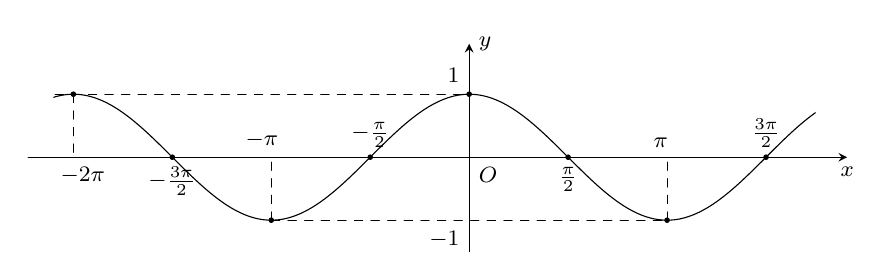
\begin{tikzpicture}[scale=0.8,>=stealth, font=\footnotesize, line join=round, line cap=round]
				\def\xmin{-10} \def\xmax{10.5} \def\ymin{-1.5} \def\ymax{1.8}
				\draw[->] (-7,0)--(6,0) node [below]{$x$};
				\draw[->] (0,\ymin)--(0,\ymax) node [right]{$y$};
				\node at (0,0) [below right]{$O$};
				\clip (\xmin+3.4,\ymin+0.1) rectangle (\xmax-5,\ymax-0.1);
				\draw[smooth,samples=400,domain=\xmin:\xmax] plot(\x,{cos(\x r)});
				\draw[dashed] (\xmin,1)--(0,1) (-3.14,-1)--(3.14,-1);		
				\foreach \x in {-2*pi,-1.5*pi,-pi,-0.5*pi,0}
				{\draw[fill=black] (\x,cos \x*180/pi) circle (1pt);
					\draw[dashed] (\x,cos \x*180/pi)--(\x,0);
					\draw[fill=black] (-\x,cos -\x*180/pi) circle (1pt);
					\draw[dashed] (-\x,cos \x*180/pi)--(-\x,0);}
				\node at (0,1.3) [left]{$1$};
				\node at (0,-1.3) [left]{$-1$};
				\node at (-2*pi+0.15,0) [below]{$-2\pi$};
				\node at (-1.5*pi,0) [below]{$-\frac{3\pi}{2}$};
				\node at (-pi-0.15,0) [above]{$-\pi$};
				\node at (-0.5*pi,0) [above]{$-\frac{\pi}{2}$};
				\node at (0.5*pi,0) [below]{$\frac{\pi}{2}$};
				\node at (pi-0.1,0) [above]{$\pi$};
				\node at (1.5*pi,0) [above]{$\frac{3\pi}{2}$};
			\end{tikzpicture}
		\end{center}
	\end{enumerate} 
	
	\loigiai{
		\begin{enumerate}
			\item Ta có
			\begin{eqnarray*} 
				&-1&\leq \cos\left[\dfrac{\pi}{4}\left( 4-\dfrac{t}{3}\right) \right]\leq 1\\ &\Leftrightarrow& - 8 \leq  8\cos\left[\dfrac{\pi}{4}\left( 4-\dfrac{t}{3}\right) \right]\leq 8\\ &\Leftrightarrow& 21 \leq 29 + 8\cos\left[\dfrac{\pi}{4}\left( 4-\dfrac{t}{3}\right) \right] \leq 37\\
				&\Leftrightarrow& 21 \leq f(t)\leq 37.
			\end{eqnarray*}
			$\text{Max} f(t) = 37$ khi $\cos\left[\dfrac{\pi}{4}\left( 4-\dfrac{t}{3}\right) \right] = 1\Leftrightarrow \dfrac{\pi}{4}\left( 4-\dfrac{t}{3}\right) = k2\pi \Leftrightarrow t = 3(4-8k)$.\\
			Do $0\leq t \leq 24$ cho nên $-\dfrac{1}{2}\leq k \leq \dfrac{1}{2}$, $k\in\mathbb{Z}$ ta chọn $k = 0 \Rightarrow t = 12$.\\ 
			Vậy nhiệt độ cao nhất trong ngày là $37$ độ C vào lúc $12$ giờ.
			\item 
			\begin{center}
				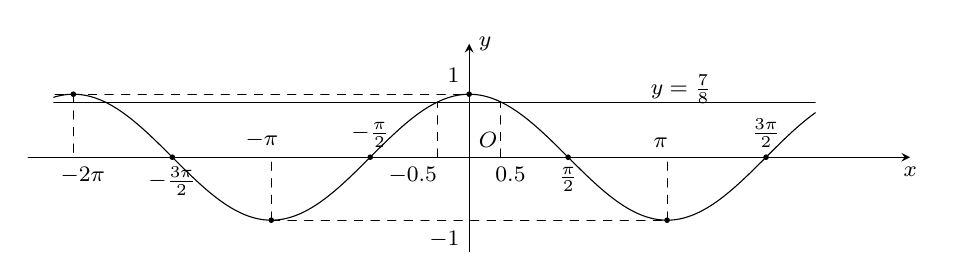
\begin{tikzpicture}[scale=0.8,>=stealth, font=\footnotesize, line join=round, line cap=round]
					\def\xmin{-10} \def\xmax{10.5} \def\ymin{-1.5} \def\ymax{1.8}
					\draw[->] (-7,0)--(7,0) node [below]{$x$};
					\draw[->] (0,\ymin)--(0,\ymax) node [right]{$y$};
					\node at (0,0) [above right]{$O$};
					\clip (\xmin+3.4,\ymin+0.1) rectangle (\xmax-5,\ymax-0.1);
					\draw[smooth,samples=400,domain=\xmin:\xmax] plot(\x,{cos(\x r)});
					\draw[dashed] (\xmin,1)--(0,1) (-3.14,-1)--(3.14,-1);
					\draw
					(\xmin,7/8)--(\xmax,7/8);
					\foreach \x in {-2*pi,-1.5*pi,-pi,-0.5*pi,0}
					{\draw[fill=black] (\x,cos \x*180/pi) circle (1pt);
						\draw[dashed] (\x,cos \x*180/pi)--(\x,0);
						\draw[fill=black] (-\x,cos -\x*180/pi) circle (1pt);
						\draw[dashed] (-\x,cos \x*180/pi)--(-\x,0);}
					\node at (0,1.3) [left]{$1$};
					\node at (0,-1.3) [left]{$-1$};
					\node at (-2*pi+0.15,0) [below]{$-2\pi$};
					\node at (0.161*pi+0.15,0) [below  ]{$0.5$};
					\node at (-0.161*pi+0.15,0) [below left ]{$-0.5$};
					\node at (4.0,0.7) [above left ]{$y = \frac{7}{8}$};
					\node at (-1.5*pi,0) [below]{$-\frac{3\pi}{2}$};
					\node at (-pi-0.15,0) [above]{$-\pi$};
					\node at (-0.5*pi,0) [above]{$-\frac{\pi}{2}$};
					\node at (0.5*pi,0) [below]{$\frac{\pi}{2}$};
					\node at (pi-0.1,0) [above]{$\pi$};
					\node at (1.5*pi,0) [above]{$\frac{3\pi}{2}$};
					\draw[dashed] (0.5,0)--(0.5,7/8);
					\draw[dashed] (-0.5,0)--(-0.5,7/8);
				\end{tikzpicture}
			\end{center}
			Theo đề bài ta có
			\begin{eqnarray*} 
				&f(t)& \leq 36 \\&\Leftrightarrow& 29 + 8\cos\left[\dfrac{\pi}{4}\left( 4-\dfrac{t}{3}\right) \right] \leq 36\\ &\Leftrightarrow & \cos\left[\dfrac{\pi}{4}\left( 4-\dfrac{t}{3}\right) \right] \leq \dfrac{7}{8}\\& \Leftrightarrow& -0{,}5  \leq \dfrac{\pi}{4}\left( 4-\dfrac{t}{3}\right) \leq 0{,}5\\& \Leftrightarrow& 10{,}1 \leq t \leq 13{,}9.
			\end{eqnarray*}
		\end{enumerate}
		
		Như vậy để tránh nhiệt độ trên $36^\circ$C thì các công nhân làm việc từ $10{,1}$ giờ đến $13{,}9$ giờ.
	}
\end{ex}
% Phương trình LG 1 VD
\begin{ex}[Trích đề thi HKI - THPT Nguyễn Khuyến - HCM - năm học 2023-2024]%[1D1C5-5]%[Dự án D - đợt 4 NH25-26- Nguyễn Trần Anh Tuấn]
	Cho phương trình $4\left(\sin^4 x+\cos^4 x \right)-8\left(\sin^6 x+\cos^6 x \right)-4\sin^2 4x=m$ trong đó $m$ là tham số. Tìm tất cả giá trị nguyên của tham số $m$ để phương trình có nghiệm.
	\loigiai{
		\begin{eqnarray*}
			&&4\left(\sin^4 x+\cos^4 x\right)-8\left(\sin^6 x+\cos^6 x \right)-4\sin^2 4x=m\\
			&\Leftrightarrow& 4\left(1-\dfrac{1}{2}\sin^2 2x\right)-8\left(1-\dfrac{3}{4}\sin^2 2x \right)-4\left(1-\cos^4 4x \right)=m\\
			&\Leftrightarrow&4\cos^2 4x+4\sin^2 2x-8-m=0\\
			&\Leftrightarrow& 4\cos^2 4x-2\cos 4x-6-m=0.\,(1)
		\end{eqnarray*}\tagEX{(1)}
		Đặt $t=\cos 4x\Rightarrow t\in [-1;1]$.\\
		$(1)$ trở thành $4t^2-2t-6-m=0\,(2)$ có $\Delta'=25+4m$.\\
		$(1)$ có nghiệm $\Leftrightarrow (2)$ có nghiệm thỏa $t\in [-1;1]$.\\
		Nếu $\Delta'=0\Leftrightarrow m=-\dfrac{25}{4}$, $(2)$ có nghiệm kép $t=\dfrac{1}{4}\in[-1;1]$ nên nhận $ m=-\dfrac{25}{4}$.\\
		Nếu $\Delta'>0\Leftrightarrow m>-\dfrac{25}{4}$, khi đó $(2)$ phải có $2$ nghiệm phân biệt thỏa 
		\[ \hoac{&-1\le t_1\le 1\\&-1\le t_2\le 1}
		\Leftrightarrow \hoac{&-1\le\dfrac{1-\sqrt{25+4m}}{4}\le 1\,(a)\\&-1\le\dfrac{1+\sqrt{25+4m}}{4}\le 1\,(b).}\]\\
		Giải $(a)$: $(a)\Leftrightarrow \heva{&1-\sqrt{25+4m}\ge -4\\&1-\sqrt{25+4m}\le4}\Leftrightarrow \heva{&\sqrt{25+4m}\le 5\\&\sqrt{25+4m}\ge-3}\Leftrightarrow\heva{&m\le 0\\&m\ge -\dfrac{25}{4}}\Leftrightarrow -\dfrac{25}{4}\le m\le 0$.\\
		Giải $(b)$: $(b)\Leftrightarrow \heva{&1+\sqrt{25+4m}\ge -4\\&1+\sqrt{25+4m}\le4}
		\Leftrightarrow \heva{&\sqrt{25+4m}\ge -5\\&\sqrt{25+4m}\le3}
		\Leftrightarrow\heva{&25+4m\ge 0\\&25+4m\le9}\Leftrightarrow -\dfrac{25}{4}\le m\le -4$.\\
		Kết hợp lại, $(1)$ có nghiệm khi $-\dfrac{25}{4}\le m\le0 $.
	}
\end{ex}